NDN~\cite{zhang2014named,afanasyev2018brief} shifts networking from a host-centric to a data-centric communication model.  In this section, we briefly review NDN and two NDN-based mechanisms used by NDNSF.

\subsection{NDN in a Nutshell}

\begin{figure}[]
    \centering
    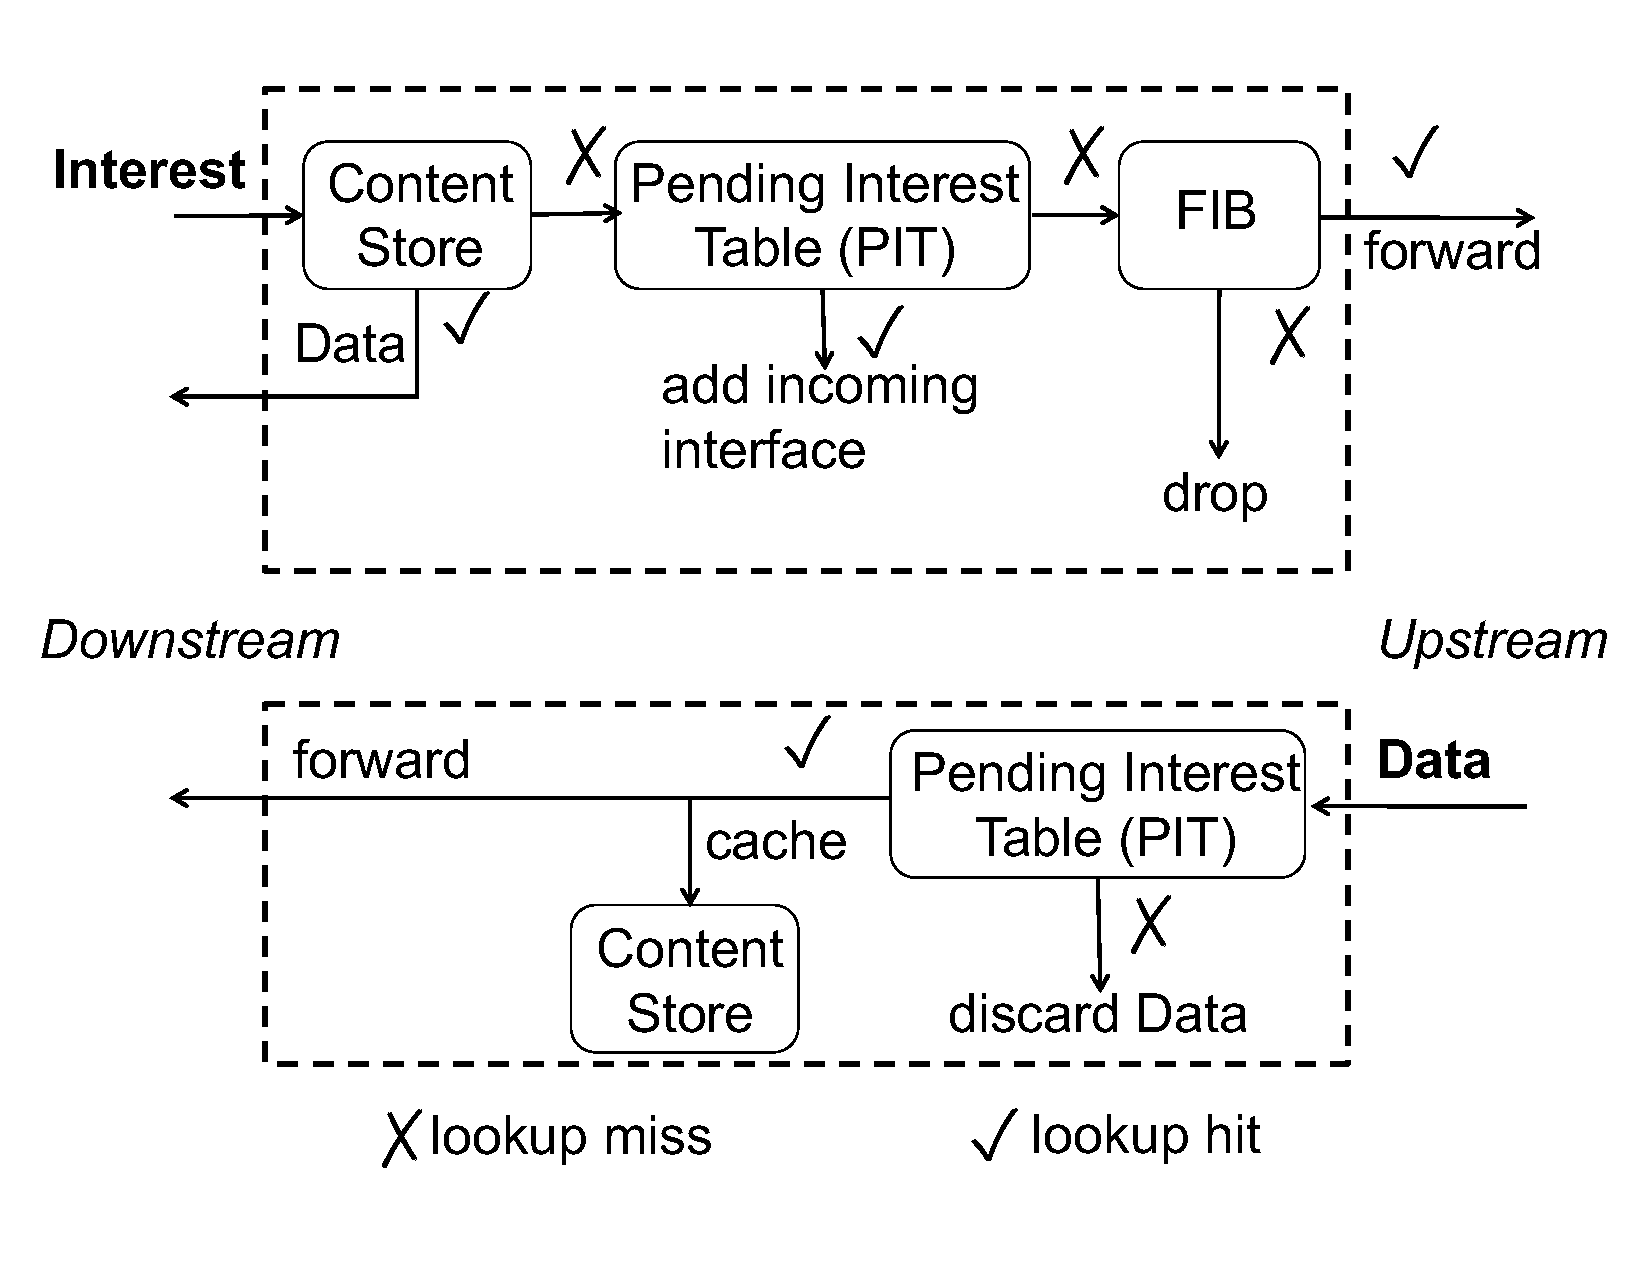
\includegraphics[width=.9\columnwidth]{figures/ndn-forwarder.pdf}
    \vspace{-3mm}
    \caption{NDN Forwarding Process (adapted from~\cite{afanasyev2018brief}, Fig.~3)}
    \label{fig:ndn-forwarder}
    \vspace{-3mm}
\end{figure}

NDN employs a receiver-driven request-response model based on two packet types: \textit{Interest} and \textit{Data}. A consumer sends an Interest packet specifying the desired data name, and the network forwards the Interest toward potential data sources using the data name, including producers and in-network caches. Once a matching Data packet is located, it is returned along the reverse path established by the Interest.

To support this process, each NDN forwarder maintains three data structures: Forwarding Information Base (FIB), Pending Interest Table (PIT), and Content Store (CS). The FIB stores name-prefix routes used by the forwarding strategy, the PIT tracks pending Interests and can aggregate compatible Interests so that a matching Data packet can satisfy multiple consumers, thereby enabling multicast delivery, and the CS caches Data packets for future requests, which can reduce retrieval latency and bandwidth consumption. Figure~\ref{fig:ndn-forwarder} illustrates how these structures operate during Interest and Data forwarding. By decoupling data from network locations and maintaining PIT state, NDN naturally enables in-network caching, multicast data delivery, and adaptive forwarding~\cite{yi2013case}.  It can also support content delivery networks (CDNs), mobile ad-hoc networking (MANET), and delay-tolerant networking (DTN)~\cite{afanasyev2018brief}.

NDN also adopts a data-centric security model in which each Data packet carries a signature. A producer's cryptographic signature, validated under trust-schema rules specifying authorized signing keys~\cite{yu2015trust}, enables consumers to verify data authenticity and integrity independently of the communication path or retrieval source, which is particularly advantageous in environments with caching and replicated content.

\subsection{NDN Sync}

In a multi-party distributed NDN application, the participants need to learn the names of data newly produced by others, so that they can retrieve new data promptly.  This functionality is provided by Distributed Dataset Synchronization, or Sync in short (\cite{li2018brief,moll2022sok}). Instead of relying on a central node, Sync participants exchange summaries of their data names and discover differences (i.e., new data names). A number of NDN Sync protocols have been developed over the last decade, such as ChronoSync~\cite{zhu2013let}, PSync~\cite{zhang2017scalable}, and State Vector Sync (SVS)~\cite{moll2021svs}. NDNSF builds on Sync to announce service-message publications without centralized coordination. In particular, we use the NDN-SVS implementation~\cite{ndnsvs-github}.

%\subsection{NDN Service Discovery (NDNSD)}
%TODO: add more details (those relevant to our paper) about how NDNSD works 
% Service discovery is crucial for modern distributed applications, and NDNSD \cite{dulal2022ndnsd} addresses this by offering a fully distributed and scalable service discovery protocol for NDN, utilizing NDN's data synchronization capabilities for efficient service publishing and discovery without external infrastructure dependencies.

\subsection{NAC-ABE}

\begin{figure}[]
    \centering
    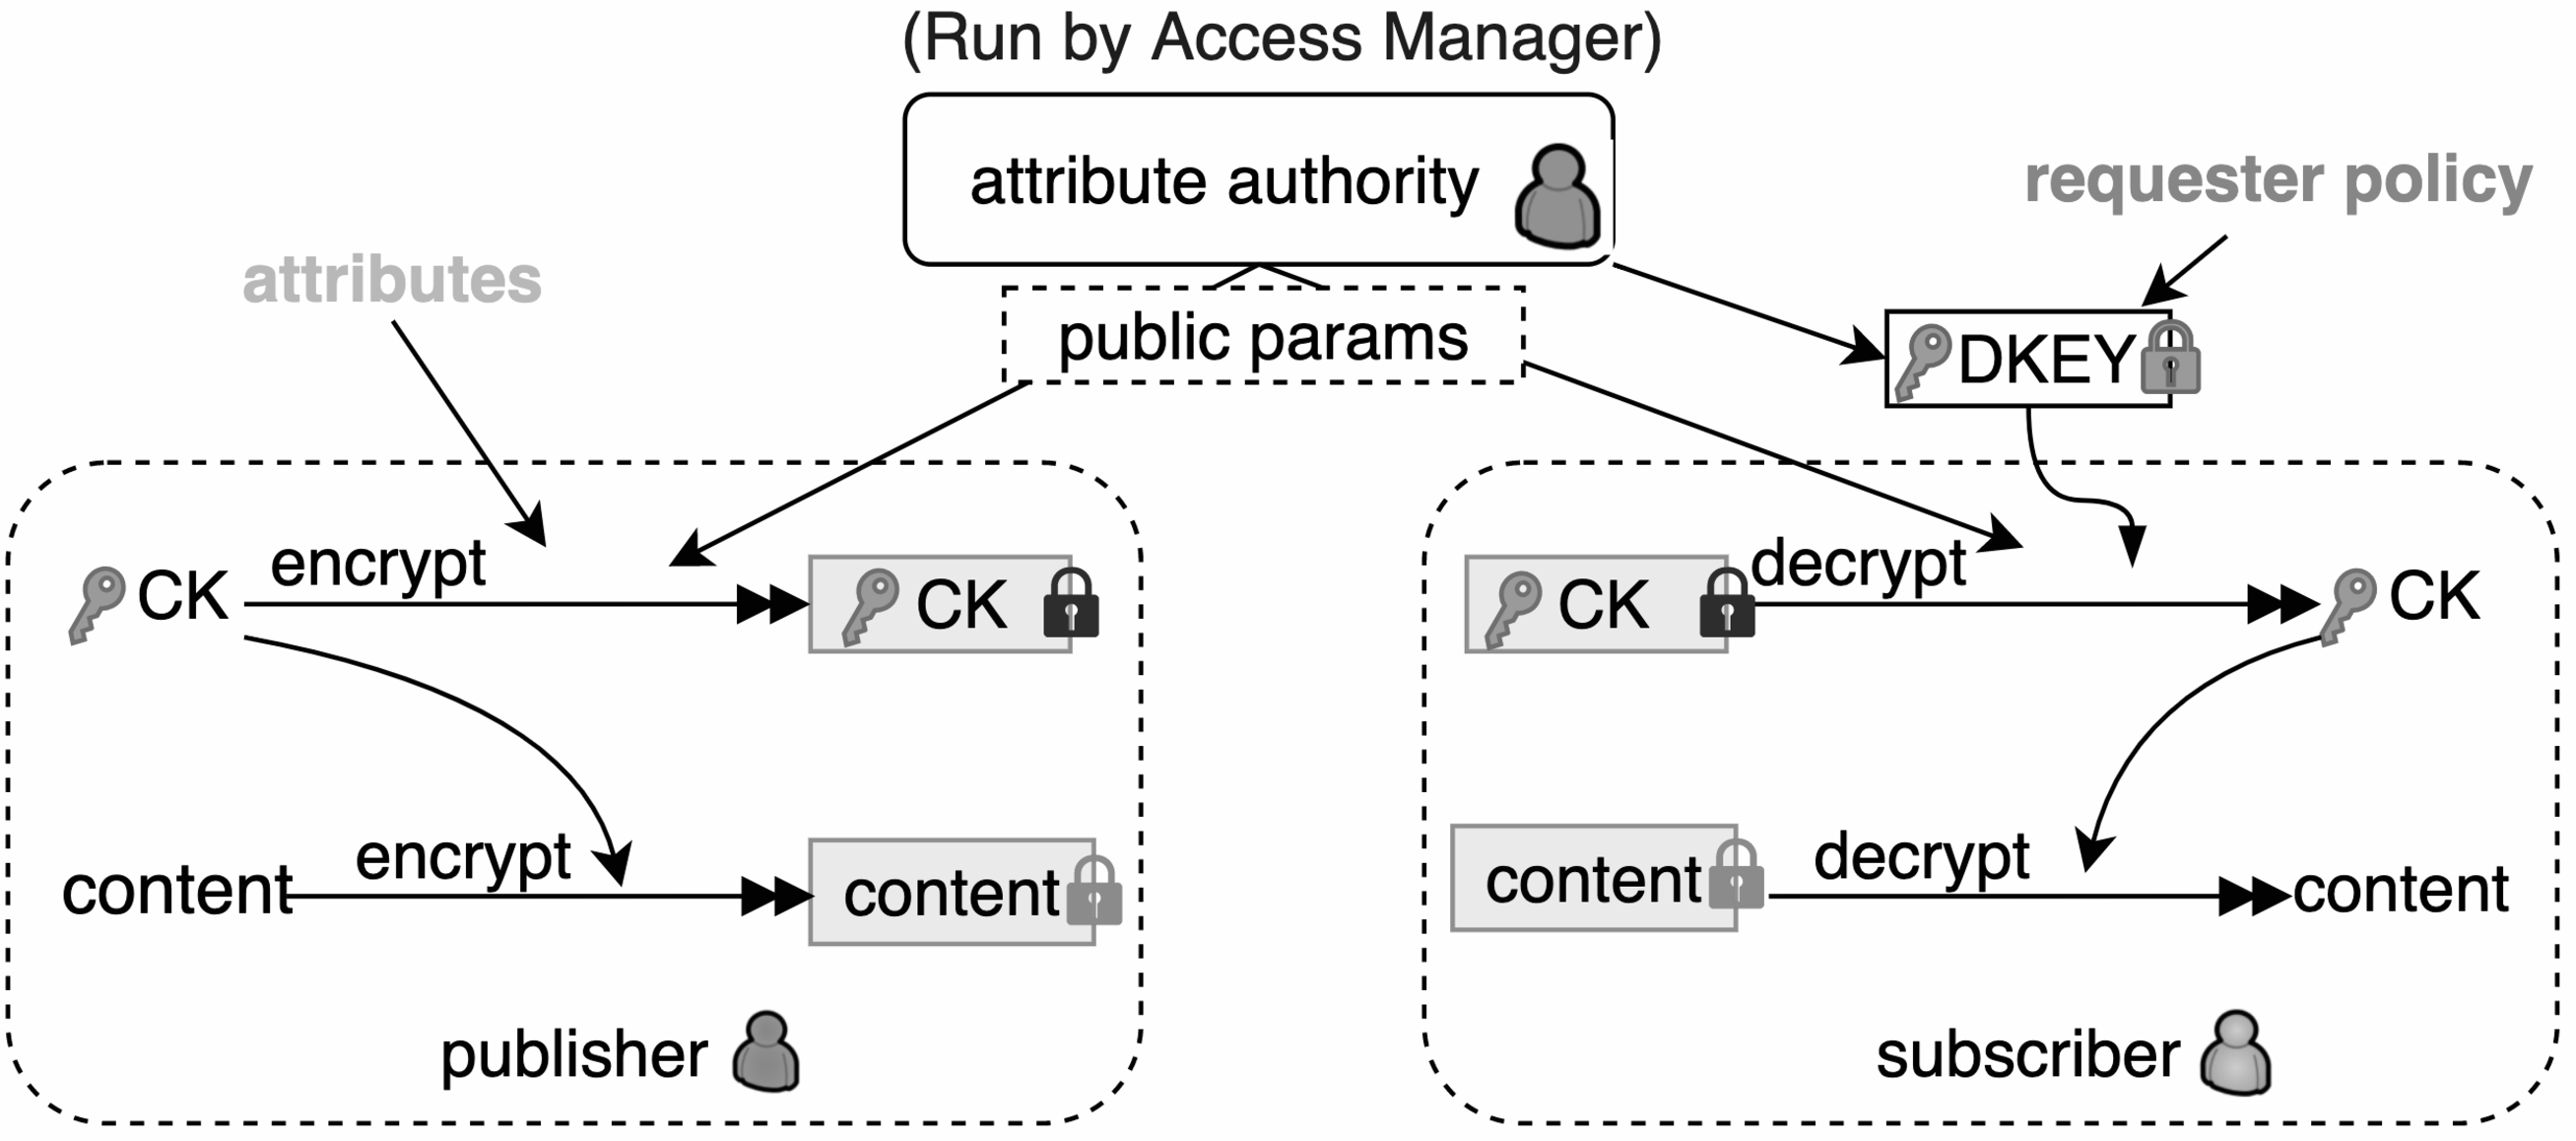
\includegraphics[width=.9\columnwidth]{figures/kp-abe-scheme.pdf}
    \caption{Encryption and Decryption with KP-ABE~\cite{dulal2023nac-abe}}
    \label{fig:kp-abe}
    \vspace{-3mm}
\end{figure}

NAC automates access-key distribution for named Data~\cite{zhang2018nac}. NDNSF leverages NAC-ABE~\cite{dulal2023nac-abe} to provide fine-grained access control and automated key management.
More specifically, we use Key-Policy Attribute-Based Encryption (KP-ABE)~\cite{goyal2006attribute} provided by NAC-ABE, where data is encrypted under a set of attributes, and each user’s decryption key (DKEY) encodes an access policy over those attributes.

In NAC-ABE, an Attribute Authority manages system attributes and issues decryption keys for access control (Figure~\ref{fig:kp-abe}). During initialization, it generates public parameters and a master secret key. The public parameters are distributed to all participants for use in cryptographic operations, while the master key is kept by the Attribute Authority to generate user-specific decryption keys (DKEYs) according to their authorized access policies.  Each data object is encrypted using a symmetric Content Key (CK), and the CK is then encrypted using ABE under the data object’s associated attributes. When retrieving data, a participant first obtains the encrypted CK (whose name is included in the data object), then decrypts it using their DKEY. The recovered CK is subsequently used to decrypt the data object itself. This hybrid design improves efficiency by applying expensive ABE operations only to the small CK, while using fast symmetric encryption for the bulk data. DKEY size can grow with policy complexity and may require segmentation~\cite{dulal2023nac-abe}.

%Each DKEY is encrypted using the corresponding participant's public key. The encrypted DKEY is packaged into an NDN data object and named according to specific conventions. Each participant retrieves the appropriate encrypted DKEY packet using these naming conventions and decrypts it with their private key to obtain their DKEY.


%\subsubsection{Bloom Filter}
%A Bloom filter \cite{lu2005bloom} is a probabilistic data structure, and it efficiently represents a set of elements and allows for fast membership queries with minimal space requirements. While it may occasionally produce false positives, it never produces false negatives, making it suitable for applications where false positives are acceptable but false negatives are not.

%\subsubsection{Protocol Buffers}
%Protocol Buffers (protobuf) \cite{protobuf_dev} is a language-neutral and platform-neutral method to serialize structured data, offering a simple and efficient way to define data formats. With protobuf, developers can define the structure of their data using a simple interface definition language and generate code in various programming languages to serialize and deserialize data in a compact and efficient binary format.
